%%%%% Introduction %%%%%
\section{Evaluation}
\subsection{Sustainability}
Sustainability in the context of compact continuum robotics manipulators, particularly those used in therapeutic 
ultrasound applications, encapsulates not only the environmental impact of manufacturing and using such devices 
but also their role in promoting sustainable healthcare practices. The novel design and application of continuum 
robots, as discussed in the article, offer significant advancements in minimally invasive surgeries and therapeutic 
treatments. These robots' high precision, flexibility, and ability to navigate complex anatomical structures reduce 
the need for large, invasive surgical interventions, leading to shorter hospital stays and faster recovery times for 
patients. This directly contributes to reducing the overall environmental footprint of healthcare by minimizing energy 
consumption, medical waste, and the use of disposable medical supplies.

Moreover, the materials selection and manufacturing methods for these robots focus on durability and efficiency. Utilizing 
advanced fabrication techniques such as multi-material 3D printing not only allows for the creation of more complex and 
tailored designs but also potentially reduces waste during the production process. The selection of materials that balance 
rigidity, flexibility, and durability contributes to the longevity of the devices, thereby reducing the need for frequent 
replacements and the associated environmental impact. 

The research and development of continuum robots also open pathways for innovations in renewable energy and environmental 
monitoring applications, further extending their sustainability impact. For instance, their flexible and adaptable design 
could be employed in underwater environments for repairing or maintaining renewable energy installations, such as tidal 
or wind turbines, without the need for large and invasive machinery. Additionally, their capacity for precise operation 
in delicate environments makes them suitable for environmental monitoring and data collection, aiding in the conservation 
of ecosystems and biodiversity. 

In conclusion, the integration of compact continuum robotics manipulators in therapeutic ultrasound and beyond holds 
promising potential for enhancing sustainability within healthcare and other sectors. By reducing the environmental 
impact of medical procedures, improving the efficiency of renewable energy maintenance, and contributing to environmental 
conservation efforts, these innovative robotic systems embody a step forward in the pursuit of sustainable technology solutions. 

\subsection{Needs Satisfaction}
\subsubsection{Societal Needs}
This project addresses the absence of fundamental open-source project about continuum manipulator in societal demand. 
Most existing open-source projects predominantly concentrate on specific aspects of soft robotics or limit their scope 
to algorithm derivation. In contrast, this project extends beyond algorithm derivation to encompass a comprehensive 
set of elements, including structural models, strength analysis, electronic control programmes, and detailed operational 
guidelines. This holistic approach ensures the reproducibility of the project and distinguishes it from others open-source 
projects. 

Moreover, under the MIT License, this project can be utilized for free, extending to its inclusion in commercial endeavors. 
The societal implications of this approach are unquestionably profound, fostering dual advancements in both technology and commerce.
The GitHub repository is demonstrated in Figure \ref{fig:github}.
\begin{figure}[H] % figure
    \centering 
    \captionsetup{labelsep=colon}
    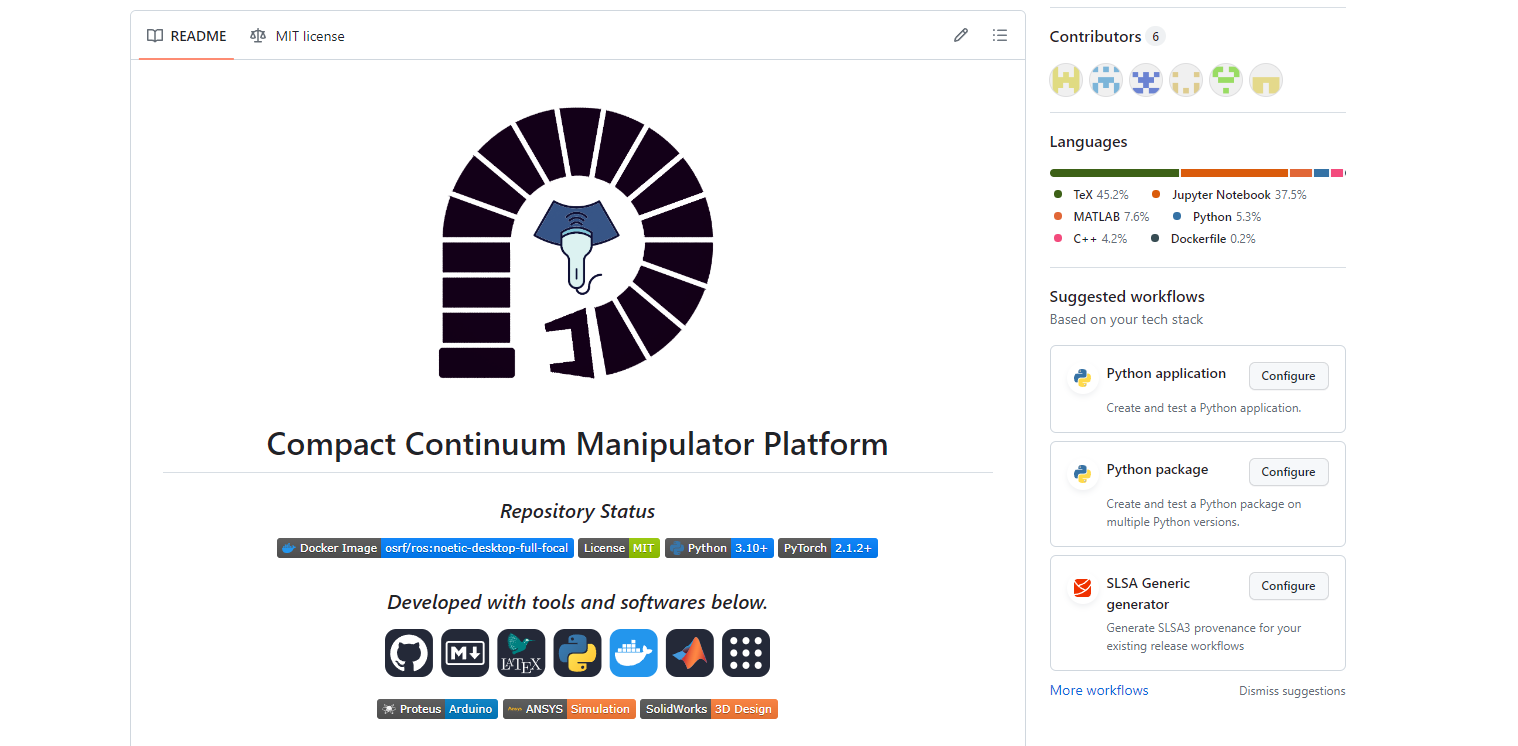
\includegraphics[width=\textwidth]{Image/Result/github.png} 
    \caption[The GitHub Repository]
    {\centering \textbf{The GitHub Repository.}}
    \label{fig:github}
\end{figure}
\vspace{-5mm}

\subsubsection{User}
From a user perspective, the workspace and payload of the continuum robot have been defined as the primary objectives to meet. 
These requirements take precedence and are given top priority. Additionally, the continuum robot incorporates a range of 
features to ensure its capability to manipulate modules accurately and assist users in corresponding operations. Simultaneously, 
the mechanical arm offers various operating modes, enhancing diversity for users during the utilization process.



% newpage
\newpage